%!TEX root = main.tex

\section{Related Work}
\label{sec:relatedwork}


\begin{figure*}[htbp]
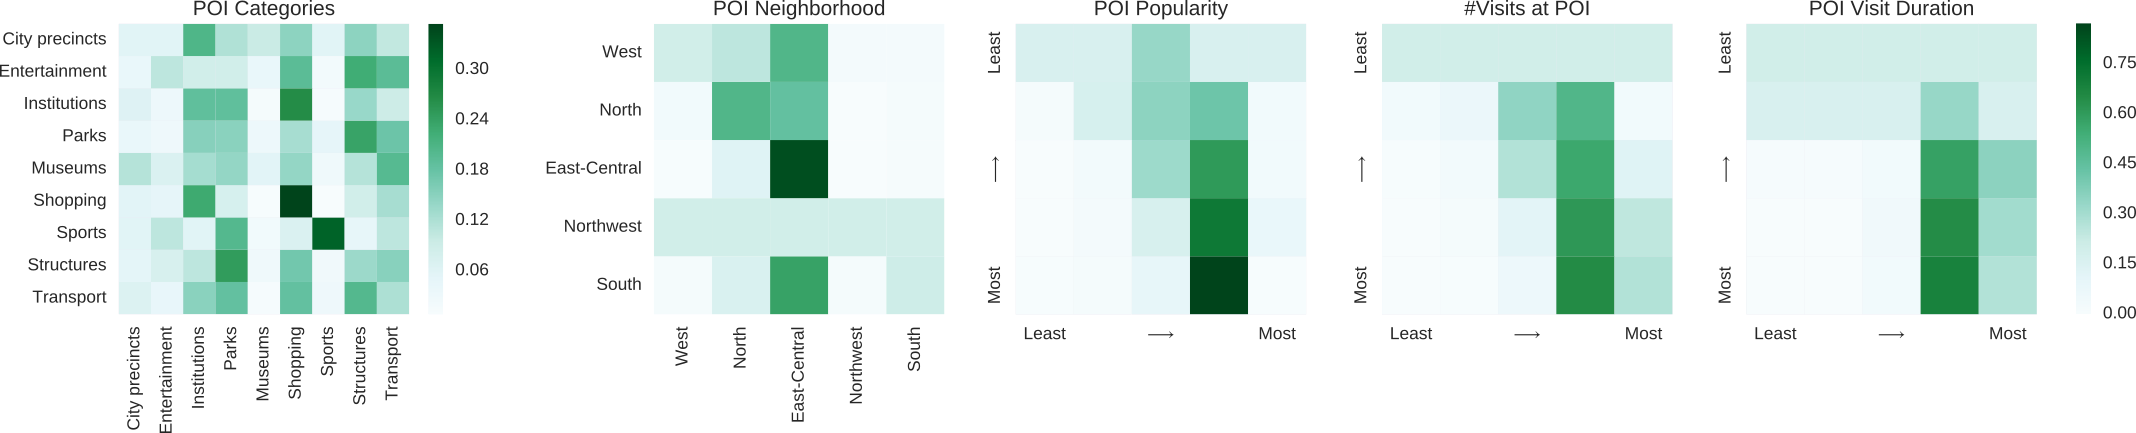
\includegraphics[width=\textwidth]{fig/poi_transmat.png}
\caption{Transition matrices for $5$ individual POI features (Melbourne)}
\label{fig:transmat}
\end{figure*}



%As geo-tagged travel data become widely available, problems in exploring routes and travel patterns has received increasing attention across several research communities -- including information retrieval and recommender systems, databases, social media, geographic information systems, and artificial intelligence.
%Exhaustive surveying of the area is beyond the scope of this work, we refer the readers to a number of
We summarise recent work most related to formulating and solving learning problems on assembling routes
from points-of-interest (POI), according to the problem setting, the method for ranking places and routes, as well as the use of different features and queries.

{\bf Problem settings} for travel patterns and trajectory data.
There are several settings of recommendation problems for locations and routes, as illustrated in Figure~\ref{fig:threesettings}.
The first setting can be called points-of-interest (POI) recommendation (Figure~\ref{fig:threesettings}(a)). Each location (A to E) is scored with geographic and behavioural information such as category, reviews, popularity, spatial information such as distance, and temporal information such as travel time uncertainty, time of the day or day of the week.
This can be in discovery mode, such as identifying points-of-interest~\cite{zheng2009mining,li2015instagram} and includes efficient querying of geographic objects for trips ~\cite{hashem2015efficient}
A popular approach is based on the collaborative filtering model
for learning user-location affinity~\cite{shi2011personalized}, with additional ways to incorporate spatial~\cite{lian2014geomf,liu2014exploiting}, or temporal~\cite{yuan2013timeaware,hsieh2014mining,gao2013temporal}, or spatial-temporal~\cite{yuan2014graph} information.
There is a rich collection of recent literature on this problem~\cite{yin2015joint,shi2011personalized,lian2014geomf,liu2014exploiting,yuan2013timeaware,hsieh2014mining,gao2013temporal,yuan2014graph}, including recent surveys~\cite{bao2015recommendations,zheng2014urban}.


Figure~\ref{fig:threesettings}(b) illustrates the second setting: next location recommendation~\cite{ijcai13,aaai16,baraglia2013learnext,zhang2015location}. Here the input is a partial trajectory (e.g. started at point A and currently at point B), the task of the algorithm is to score the next candidate location (e.g, C, D and E) based on the perceived POI score and transition compatibility with input $A\rightarrow B$.
It is a variant of POI recommendation except given both the user and locations travelled to date. The solutions to this problem include incorporating Markov chains into collaborative filtering~\cite{fpmc10,ijcai13,zhang2015location},
quantifying tourist traffic flow between points-of-interest~\cite{zheng2012patterns},
by formulating a binary decision or ranking problem~\cite{baraglia2013learnext}, or with sequence models such as recurrent neural networks~\cite{aaai16}.



This paper considers the final setting: route recommendation, as illustrated in Figure~\ref{fig:threesettings}(c). Here the input are some factors about the desired route, e.g. starting point A and end point C, along with auxiliary information such as the desired length of trip. The algorithm needs to take into account location desirability (as indicated by node size) and transition compatibility (as indicated by edge width), and compare route hypotheses such as A-D-B-C and A-E-D-C. Existing work in this area either uses heuristic combination of locations and routes~\cite{lu2010photo2trip,ijcai15,lu2012personalized}, or formulates an optimisation problem that is not informed or evaluated by behaviour history~\cite{gioniswsdm14,chen2015tripplanner}. Joint learning of locations preferences and routes remains an open problem.
Our work is in this category, we formulate a learning problem to score the whole trajectory, taking into account individual POI properties and relationships among different POIs.



%We group the methods for ranking and recommending location and trajectories into three broad categories.
{\bf Methods} for ranking locations and trajectories.
The first is collaborative filtering, or matrix factorisation family of techniques applied to places and trajectories~\cite{shi2011personalized,ijcai13,zhang2015location}. The second type regards route recommendation as a planning problem~\cite{gioniswsdm14,ijcai15}.
%Gionis et al~\cite{gioniswsdm14} formulates optimisation problems with additive user satisfaction and coverage constraints. Lim et al.~\cite{ijcai15} uses a combination of user preference and POI popularity as objective function, and then solves a travelling salesman problem (TSP) to obtain a route.
The TripBuilder system~\cite{brilhante2013shall} first solves a maximum coverage problem for user preference and then solves TSP for routing. The collaborative filtering approaches rank POI but do not take into account the sequence that a trip is taken. On the other hand, the planning approaches assume a fixed objective function that is not directly optimised to predict user behaviour. There have been a few approaches that jointly consider POI preference and routes~\cite{lu2012personalized, kurashima2010geotag,chen2015tripplanner}.
%Lu et al~\cite{lu2012personalized} uses heuristic combinations for point scoring, followed by branch-n-bound search for planning. Kurashima et al~\cite{kurashima2010geotag} modelled user preferences and his/her transition patterns between POIs using a hybrid of Markov chain and topic models, the search for a best path is done by greedily maximising the probability for the next point. The TripPlanner system~\cite{chen2015tripplanner} selects POIs based on input query and POI categories, and then scores routes using heuristic search strategies taking into account traffic and travel time constraints.
We propose a new approach that combines different POI features and POI-POI transition features, while learning the relevant weights from data. We also provide a comprehensive benchmark on how node- and edge- features contribute to the final trajectory ranking.


%planning:
%% Trip Builder
%\cite{tripbuilder15} recommended trajectories by first addressing a Generalized Maximum Coverage problem with respect to user preference and
%time budget to get a set of candidate trajectories, which were then scheduled by solving a variant of Traveling Salesman Problem to form the
%final recommendation.
%% WSDM'14
%\cite{gioniswsdm14} proposed a framework to recommend trajectories based on user provided constraints such as the visiting order of different
%categories of POIs, time and distance budget as well as the upper/lower bounds of the number of POIs in each category that a user wish
%to visit, user satisfaction at a POI was modeled by either associate a benefit or a set of other POIs and activities to that POI,
%and proved the maximization of user satisfaction is NP-hard in both cases.
%They further proposed pseudo polynomial dynamic programming algorithms as well as
%a $1-\epsilon$ approximation algorithm to maximize the user satisfaction.


%joint
%\cite{lu2012personalized} claims to do both point ranking and trip planning, heuristic combination for point scoring, branch-n-bound search for planning.
%% IJCAI'15
%Lim et al.~\cite{ijcai15} modeled user's interest on a specific category of POIs based on the observation that if a user is more interested in a certain category of POIs, his/her visit duration would be longer than the average visit duration in general. They then formulated trajectory recommendation as a Orienteering problem and use integer programming to optimize an objective which was a composite of the total POI popularity as well as the total user interest on POIs in the recommended trajectory
%with respect to a number of constraints such as the start/destination POI and time budget.
%\cite{kurashima2010geotag} modeled user preferences of POIs and his/her transition patterns
%between POIs using a hybrid of
%Markov and topic models, and recommend a trajectory by search the sequence of POIs with highest probability for %this user  with respect to a time budget.
%greedy on best next location.


%{\bf queries, features, available data}
%One of the challenges for modeling traveling behavior is the diversity of available information,
{\bf A diverse set of available information},
such as geographic, time, user properties, and subjective opinions.
Approaches for modelling space include geolocation-informed matrix factorisation~\cite{lian2014geomf}, spatial topic models~\cite{hu2013spatialtopic}, neighbourhood information~\cite{liu2014exploiting}, exploiting sequential information with additive Markov chain~\cite{zhang2014lore}, and enriching location with the information for venues~\cite{deveaud2014importance,deveaud2015experiments}.
Important variants to consider for modelling time include travel time~\cite{gao2013temporal},
constructing time-aware routes~\cite{yuan2013timeaware,hsieh2014mining}, time-of-day and day-of-week~\cite{chen2015tripplanner}, POI availability and uncertainty in travelling time~\cite{zhang2015personalized}. There are a number of approaches that jointly consider space and time\cite{yuan2014graph,zhang2015location}, such as modelling the correlation between check-in time and location~\cite{gao2013temporal}.
Inferring user attributes and preferences has been an important consideration~\cite{liu2013personalized}.
Chen et al~\cite{chen2013people} recommend places to travellers based on automatically mined user attributes
(e.g., age, gender and race) and travel group types (e.g., couple, family and friends) from online photos.
Ference et al~\cite{ference2013location} tailors the recommendation for out of town users.
Subjective opinion is an important information source for decision making, in addition to past behaviours. Zhang et al~\cite{Zhang2015OOP} use written reviews for POI recommendation.
The novel work from Quercia et al~\cite{ht14} crowd-source judgements about the beauty, quietness and happiness about places, and then constructs routes with these subjective criteria.
%aims to recommend a short and pleasant trajectory from the current POI to a destination POI by choosing the best average rank of all POIs in a trajectory from the $M$ shortest paths that connect the current location and destination,
%POIs were ranked according to the degree of pleasure based on user votes and  crowd-sourced emotion scores on three aspects
%(i.e., beauty, quietness and happiness).
In this work we focus on formulating learning problems to jointly rank POIs and routes. We use a minimum but commonly available set of features, such as neighbourhood, popularity, and venue information. Gathering additional features via data linking for the dataset is out of the scope of this paper.

%{\bf what we do:}
%trajectory recommendation, learning the joint preference of ranks routes, on minimum but commonly available set of features.


%POI rec from photos~\cite{shi2011personalized}
%``Photo2Trip: generating travel routes from geo-tagged photos for trip planning''~\cite{lu2010photo2trip}
%Estimation markov chain from regions of interest in photos~\cite{zheng2012patterns}


%\cite{ference2013location} - Location recommendation for out-of-town users
%\cite{liu2013personalized} Personalized point-of-interest recommendation by mining users' preference transition
%\cite{baraglia2013learnext} -- next

%\cite{liu2014exploiting} -- geo, neighborhood
%\cite{yuan2014graph} Graph-based point-of-interest recommendation with geographical and temporal influences
%\cite{hsieh2014mining} - time-aware routes
%\cite{deveaud2014importance} -- venue-dependent features for learning to rank contextual suggestions
%\cite{deveaud2015experiments} - Experiments with a Venue-Centric Model for Personalisedand Time-Aware Venue suggestion
%\cite{hashem2015efficient} -- Efficient Computation of Trips with Friends and Families
%\cite{zhang2015personalized} -- Personalized Trip Recommendation with POI Availability and Uncertain Traveling Time
%\cite{zhang2015location} -- Location and Time Aware Social Collaborative Retrieval for New Successive Point-of-Interest Recommendation
%\cite{yin2015joint} -- Joint modeling of user check-in behaviors for point-of-interest recommendation
